
This chapter provides important artifacts related to design of our project. It includes the Software and Data design of our project.

\section{Software Design}

% This section presents the UML class diagram and gives a brief description of each class in our system. Attributes and methods of each class and relationship among classes are clearly presented.

\begin{figure}[H]
    \centering
    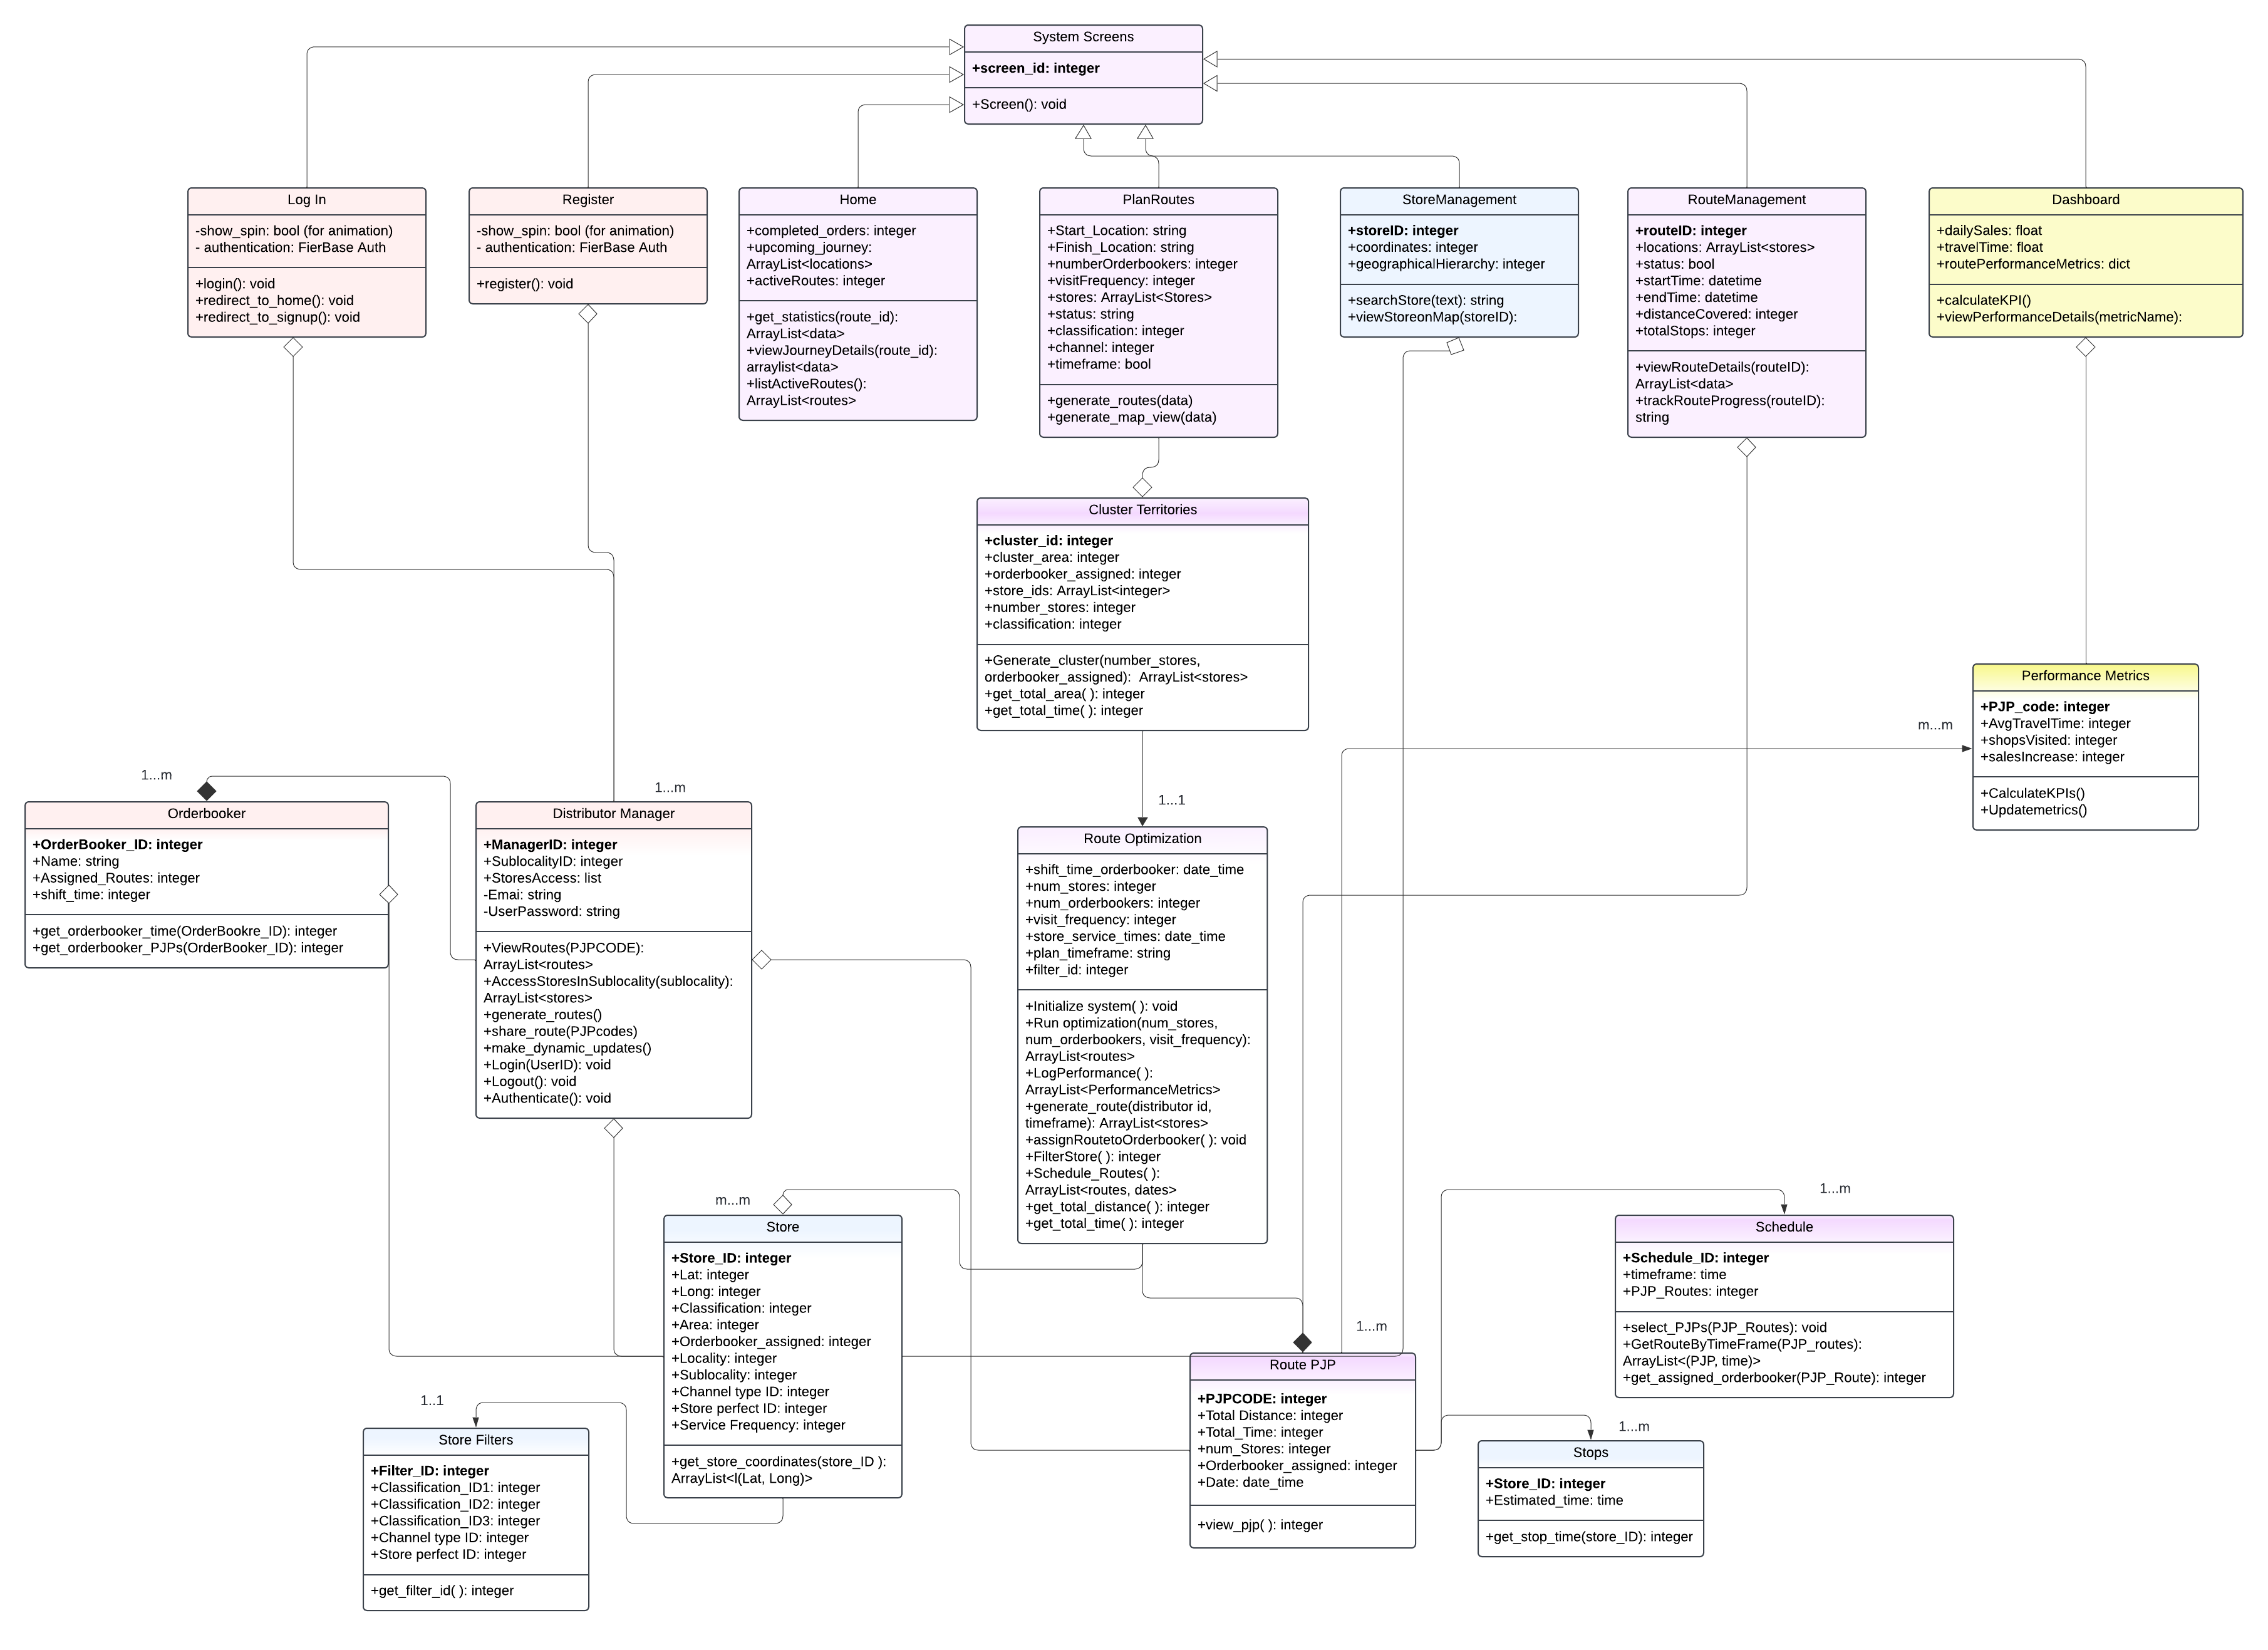
\includegraphics[width=0.9\textwidth]{images/UML class f2.png} % Adjust the width as needed
    \caption{UML Class Diagram}
    \label{fig:UML-image}
\end{figure}

% Your report will contain ONE of the following 2 sections.

As shown in Figure~\ref{fig:UML-image}, the UML diagram starts off by showing the screens that are connected to the system. The Register screen creates the object for the distributor manager, giving them access to the system and screens mentioned such as home, plan routes, route management, and etc. Next, the user has the option to Plan Routes from that screen where they give certain parameters mentioned in the attributes. This creates a cluster object for different areas containing different stores. Next, the optimal PJP route will be determined in each cluster that creates the object for clusters. After this, the stores in each cluster will be connected to form a route, creating a routes class that is the optimal PJP plan. These routes can also be viewed on a schedule view to visually analyze how the upcoming PJPs look like. Moreover, a separate stores table is connected to the child table of stores filters that provides the further classification of each store id. Lastly, the dashboard screen gets the KPIs from the Performance Metrics class to display how the performance of each PJP is and to visualize it in graphs and display the metrics.

\section{Data Design}

This section presents the structure of our database that caters to persistent data storage in our project. The structure is shown as a normalized data model for relational databases. It clearly shows entities, attributes, relationships with their cardinalities, and primary and foreign keys. We have used Postgresql ERD to build our data model.

\begin{figure}[H]
    \centering
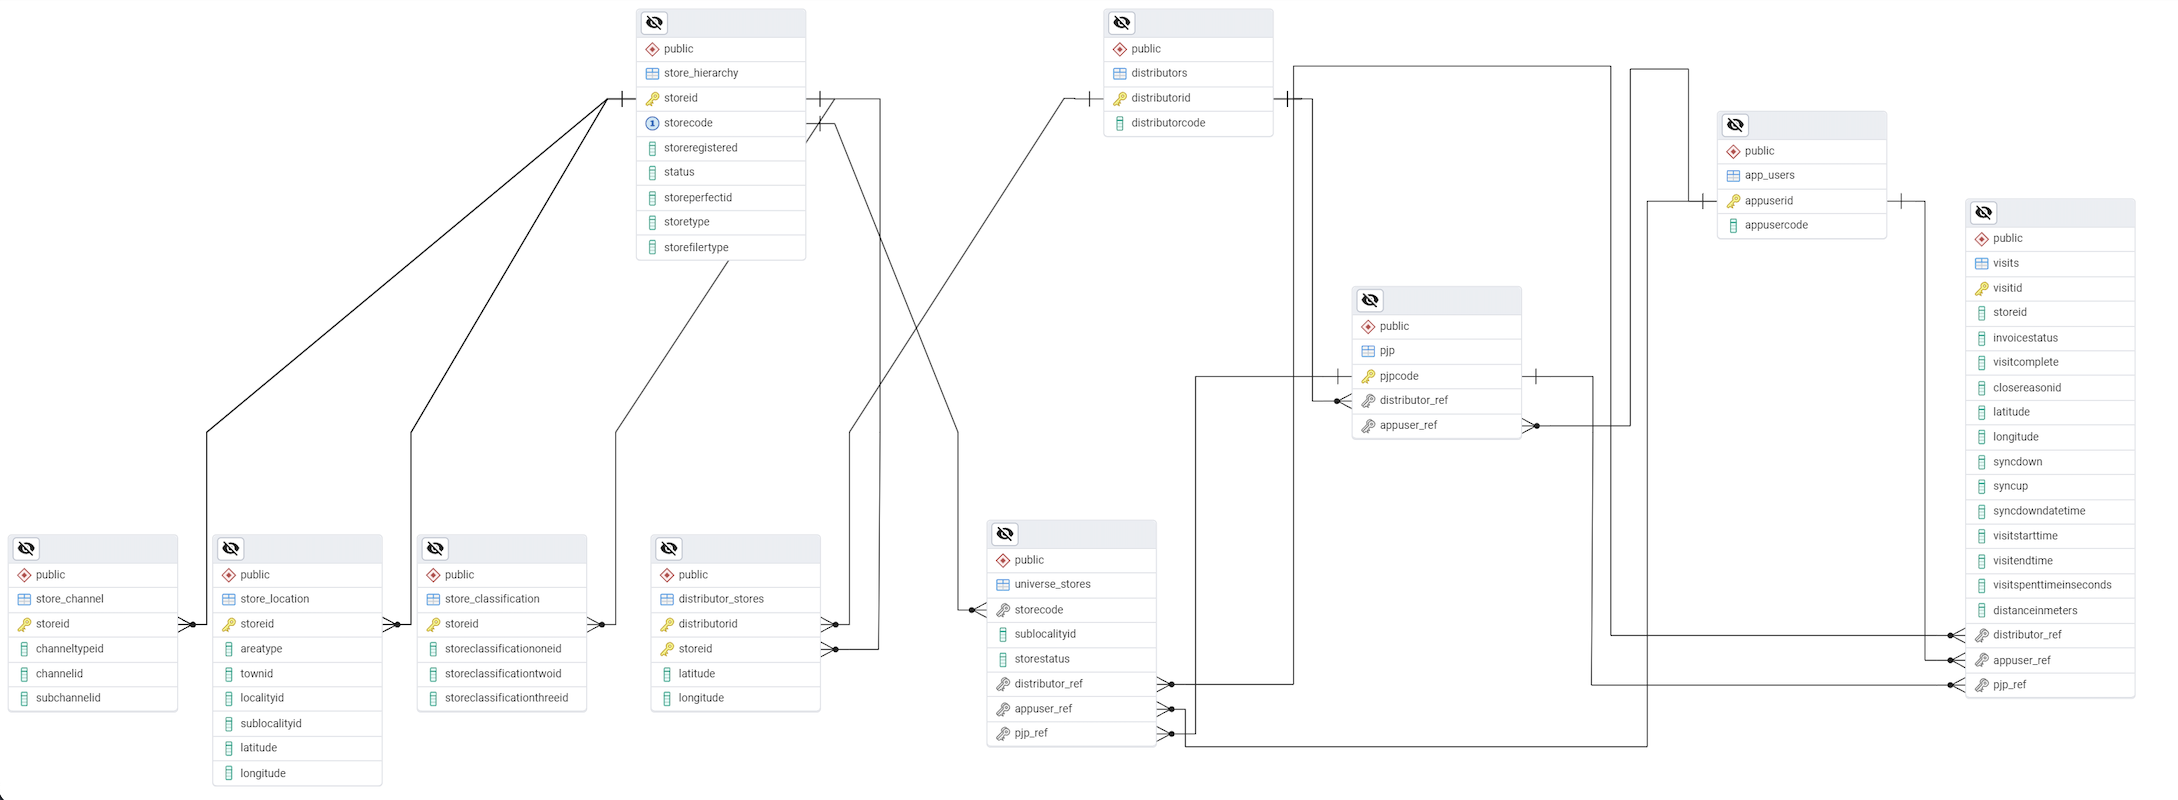
\includegraphics[width=\textwidth]{images/erd.png} % Adjust the width as needed
    \caption{ERD Diagram}
    \label{fig:UML-image}
\end{figure}
\begin{figure}[H]
    \centering
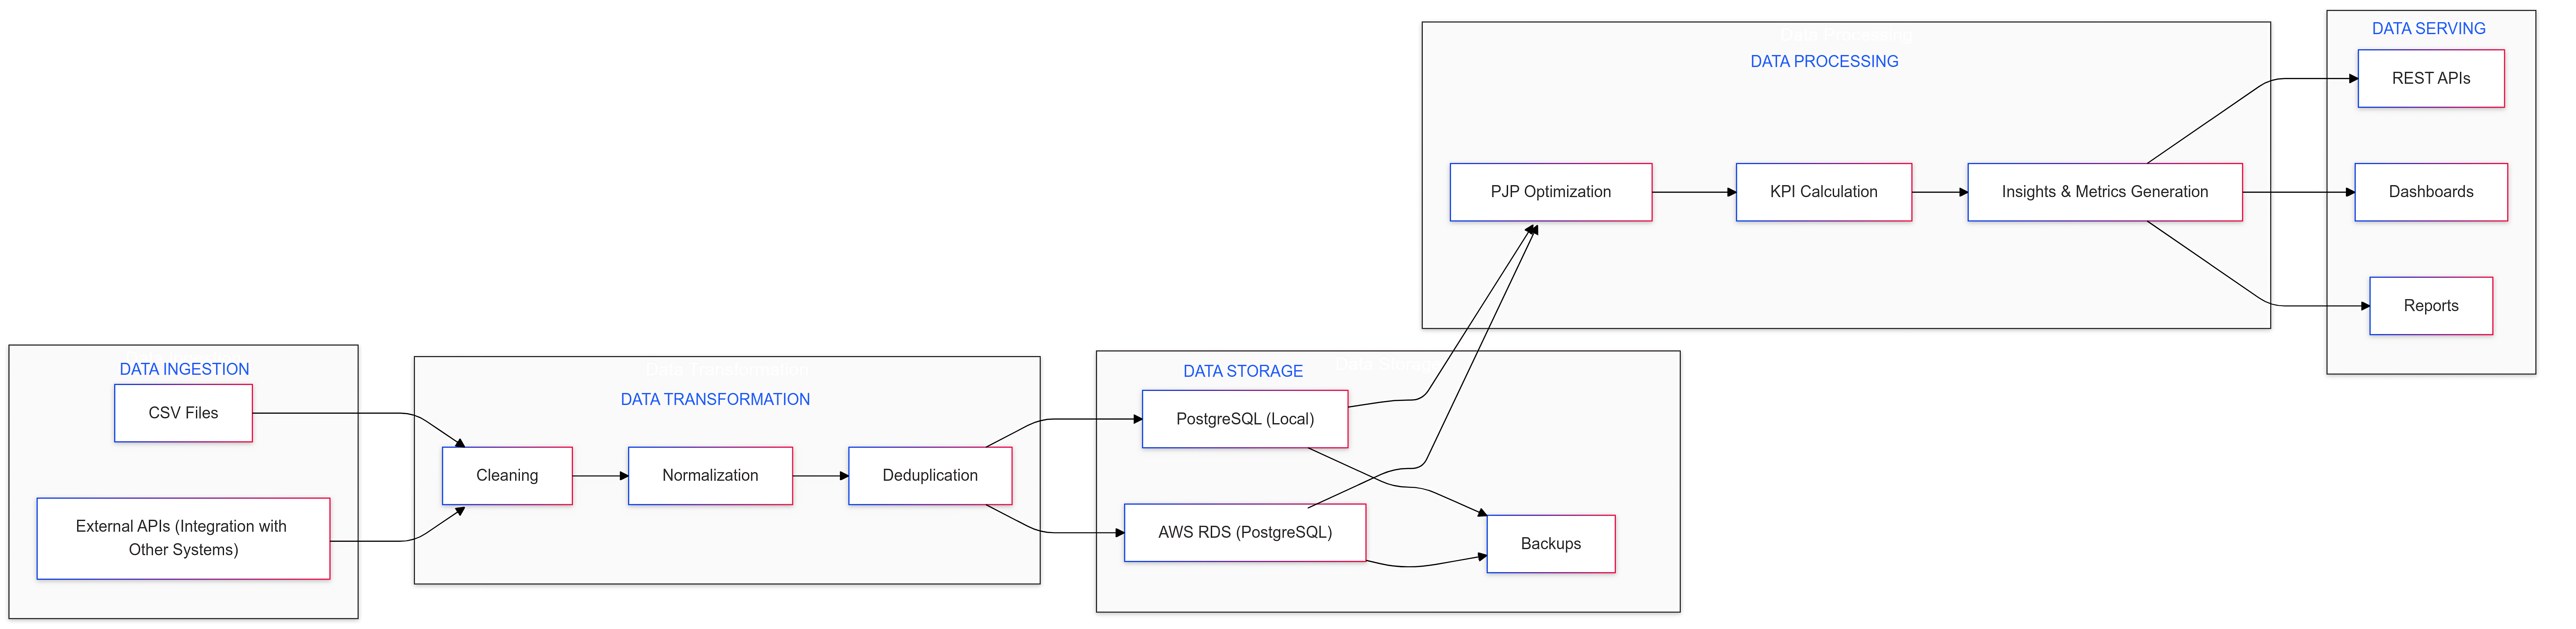
\includegraphics[width=1.1\textwidth]{images/DataPipeline (1).png} % Adjust the width as needed
    \caption{End-to-end data pipeline showcasing ingestion, transformation, storage, processing, and serving}
    \label{fig:UML-image}
\end{figure}

 
\section{Technical Details}

As shown above, our project includes an ERD created based on the cleaned data. Additionally, following are the technical aspects of the algorithm (Evolutionary Algorithm) utilized so far.
\\
The primary objectives of our algorithm are:
\begin{itemize}
    \item Maximizing the number of shops visited within the constraints.
    \item Minimizing the total distance traveled to improve route efficiency.
    \item Minimizing overall time spent, which includes travel and time spent at each store.
\end{itemize}

The constraints of our algorithm are:
\begin{itemize}
    \item \textbf{Number of order bookers}: Determines the workload distribution and affects route planning.
    \item \textbf{Shift times}: Incorporates break times, holidays, and working hours.
    \item \textbf{Duration at each store}: This is a fixed value for each visit and must be accounted for in total route time.
    \item \textbf{Store priority}: A priority metric for stores, which could be calculated based on sales data.
\end{itemize}
These objectives and constraints guide the design and functionality of our route optimization algorithm. The algorithm dynamically adapts to these parameters to give optimal route plans.